
\chapter{$O^2$ Simulations of FT0-A}
The ALICE Online-Offline Computing System $O^2$ has built-in simulation capabilities which include the generation of events and the transport of particles from the primary vertex. Using the FIT detector geometry in a simulation, we can determine the number of particles that can be detected using FIT sensitive components, and the number of secondary particles that contribute to the noise of other detectors. $O^2$ handles simulation data very similarly to true event data in the form of \textit{digits}, which only keep the location and energy deposition in the detector channel. Using this information, simulations can be used to inform live track reconstruction, background estimation, and particle identification. 


\sectionWithFixedHeader{Monte Carlo Event Simulations and Detector Geometry}{MC Simulations}

Simulations of particle physics interactions consist of three main components of simulation: event generation, particle transport, digitization. These elements of simulation are supported by specialized software that is optimized for each task. Monte Carlo simulations use computational approaches for randomized independent events; the inherent statistical nature of the events is evinced by the experimentally determined probability distribution functions, which are sampled randomly for each event. 

\subsection{Event Generation}
 Particles in the LHC are circulated in "bunches", which have a wide distribution of momentum and rapidity. To simulate the stochastic nature of events in ALICE, $O^2$ uses a Monte Carlo event generator such as PYTHIA for p-p collisions \cite{PYTHIA} or HIJING for Pb-Pb collisions \cite{HIJING}, and others for testing different kinds of physics.
 
\subsection{Particle Transport}
Particle transport is important for the next step in simulation. After an event is generated, particles are propagated away from the interaction point using experimentally determined probability distributions to simulate the passage of generated particles through the detector, modeling their energy loss in the material description of the detector.  To do this we need a geometric description of the detector. Particle transport must be optimized to handle the high volume of data produced by the particles as they pass through the detector description, which is achieved using the GEANT4 (for GEometry ANd Tracking) package\cite{Geant4}. GEANT4 has a multi-threading library that satisfies the $O^2$ speed requirements. Along with high particle transport efficiency, GEANT4 has compatibility with ROOT\cite{ROOT} geometry capabilities that allow for construction of the ALICE detector geometry in simulation.  Figure \ref{fig:GEANT_Geometry} shows the LHC Run 1 ALICE detector rendered in GEANT4 using the ROOT geometry package.  GEANT4 helps to accurately track which of the detectors are hit, which materials a particle travels through, and how much energy is deposited at each step of the transport process.  All of this information can be packaged into composite signals that mimic the information that would be provided in a real detector operating in beam.  For this project, the FT0-A support structure geometry has been implemented and will be described in the next section.

\subsection{Digitization and Reconstruction}

As particles are propagated through detector geometry, interactions that deposit energy into a material are considered \textit{hits}. Hits are implemented to contain all information from the interactions, acting as Maxwell's Demon \cite{MaxwellDemon} with a ledger of all vertices and branches that precede the hit. This information is convolved with the granularity, live-time, signal shape, and ADC characteristics of the electronics used in detector hardware, which comes from experimental hardware tests and is included in the simulation implementation. Using information from the hits and detector fidelity tests, \textit{digits} are computed. Digits contain the same information as real experimental signals and can be used to reconstruct tracks left in the detectors. This is done by comparing reconstructed tracks using the digits and experimental data, then matching reconstructed tracks with the simulated hits. 

\begin{figure}[H]
    \centering
    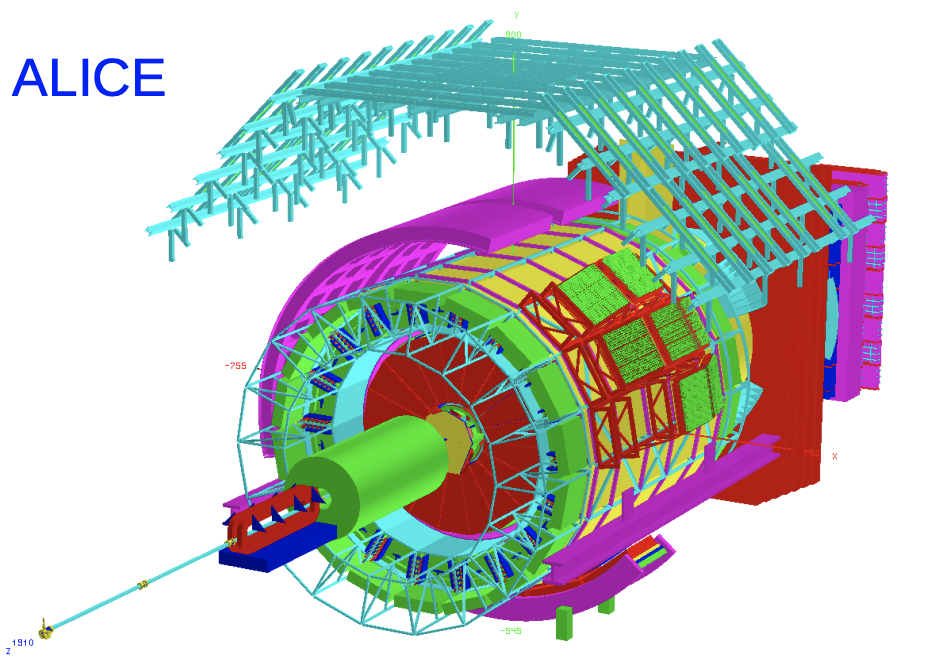
\includegraphics[width=0.6\textwidth]{figures/ALICE/GEANT_Geometry.png}
    \caption{RUN 1 ALICE detector geometry implemented in Geant4\cite{alice_geant} }
    \label{fig:GEANT_Geometry}
\end{figure}


\sectionWithFixedHeader{FT0-A Aluminum Support Structure $O^2$ Implementation}{FT0-A Aluminum  Support}
CAD drawings of the final design for the FIT FT0-A support structure, shown in Figure \ref{fig:FT0_CAD}, were completed in summer of 2019, and the support structure needed to be included in the simulation geometry. Using ROOT's geometry description software, the structure was implemented into the $O^2$ FT0 class, and is now included in simulations of FT0.  Figure \ref{fig:FT0_Labels} shows the description of the detector component labeling scheme for FT0-A and FT0-C.

\begin{figure}[H]
    \centering
    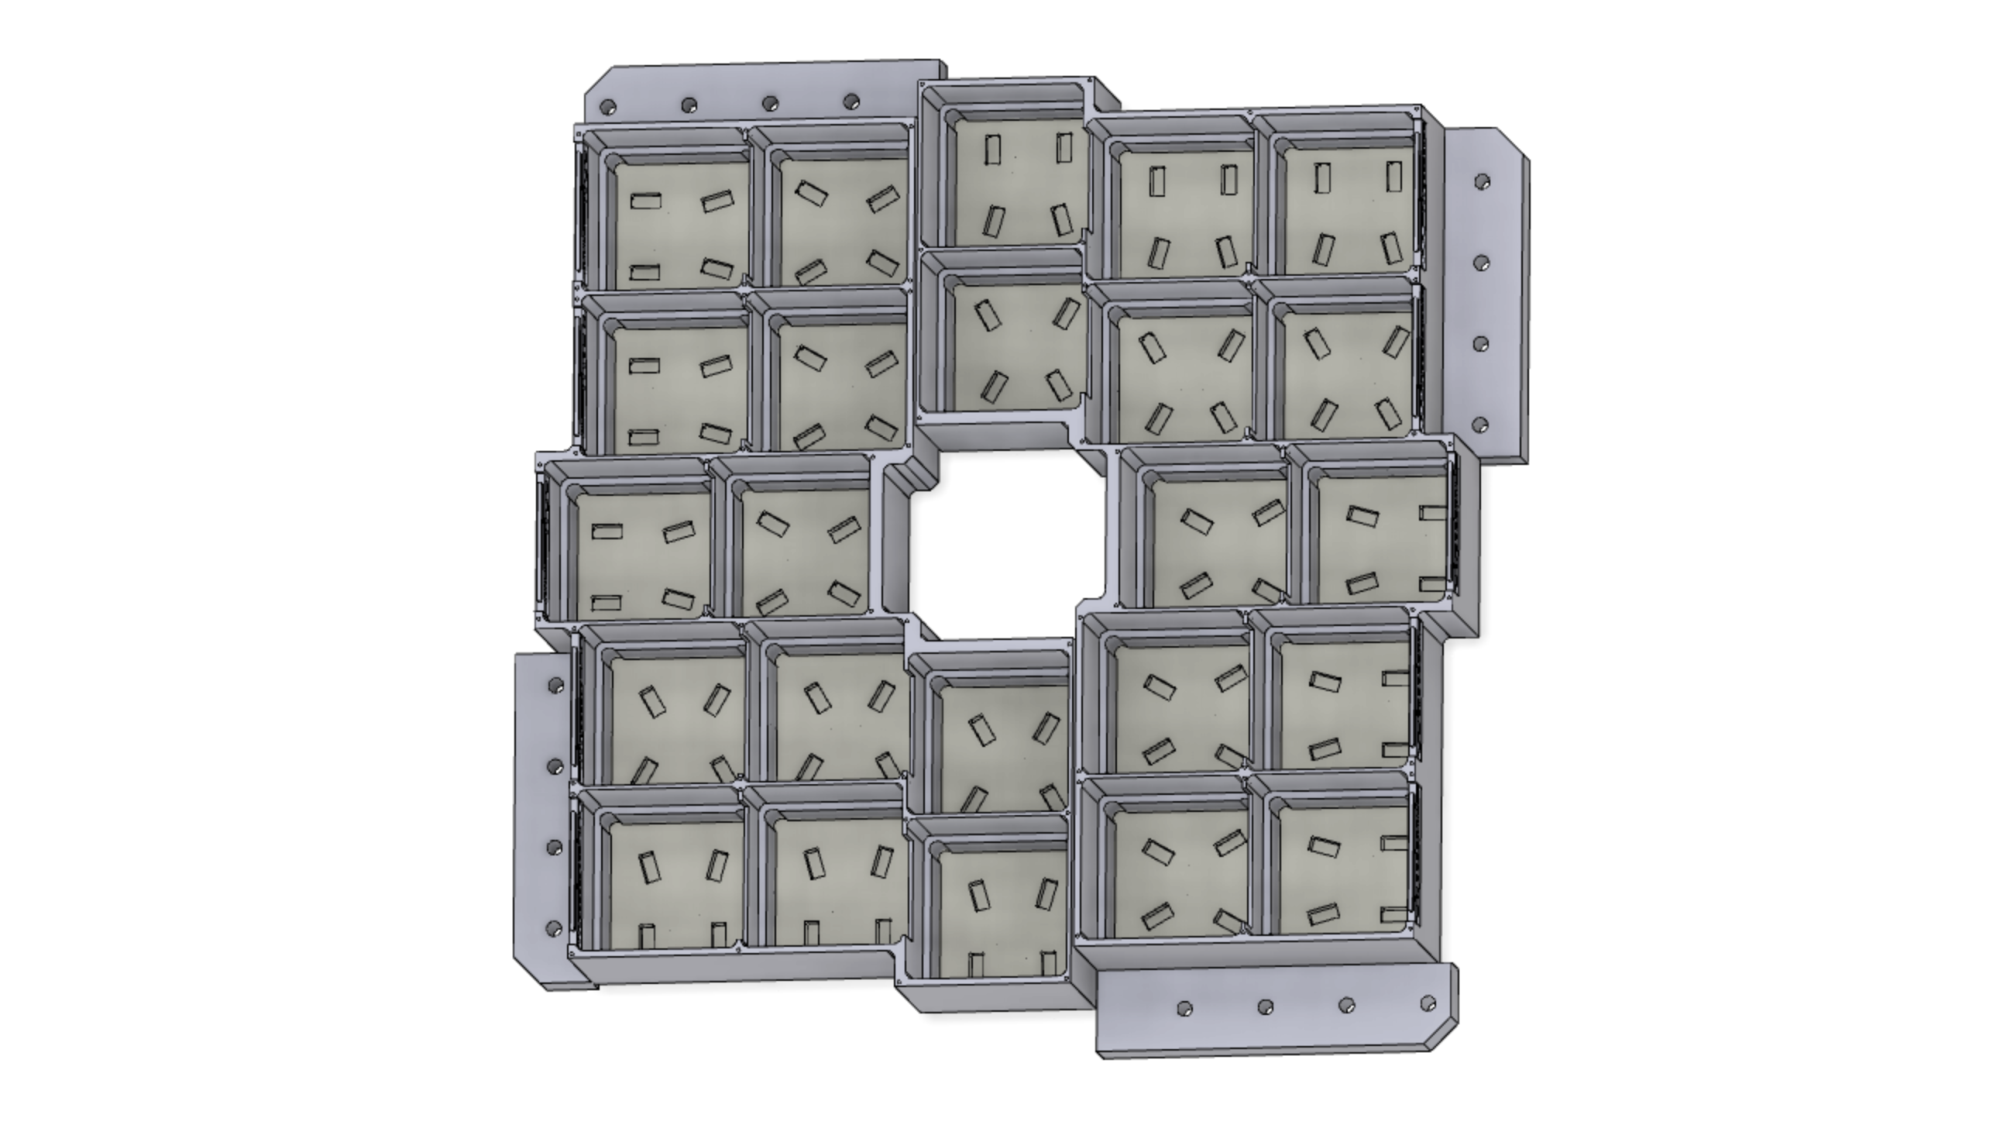
\includegraphics[width=0.6\textwidth]{figures/FIT/FIT_Support_Structure_CAD.pdf}
    \caption{CAD drawing of Aluminum support structure for FT0-A.}
    \label{fig:FT0_CAD}
\end{figure}

\begin{figure}[H]
    \centering
    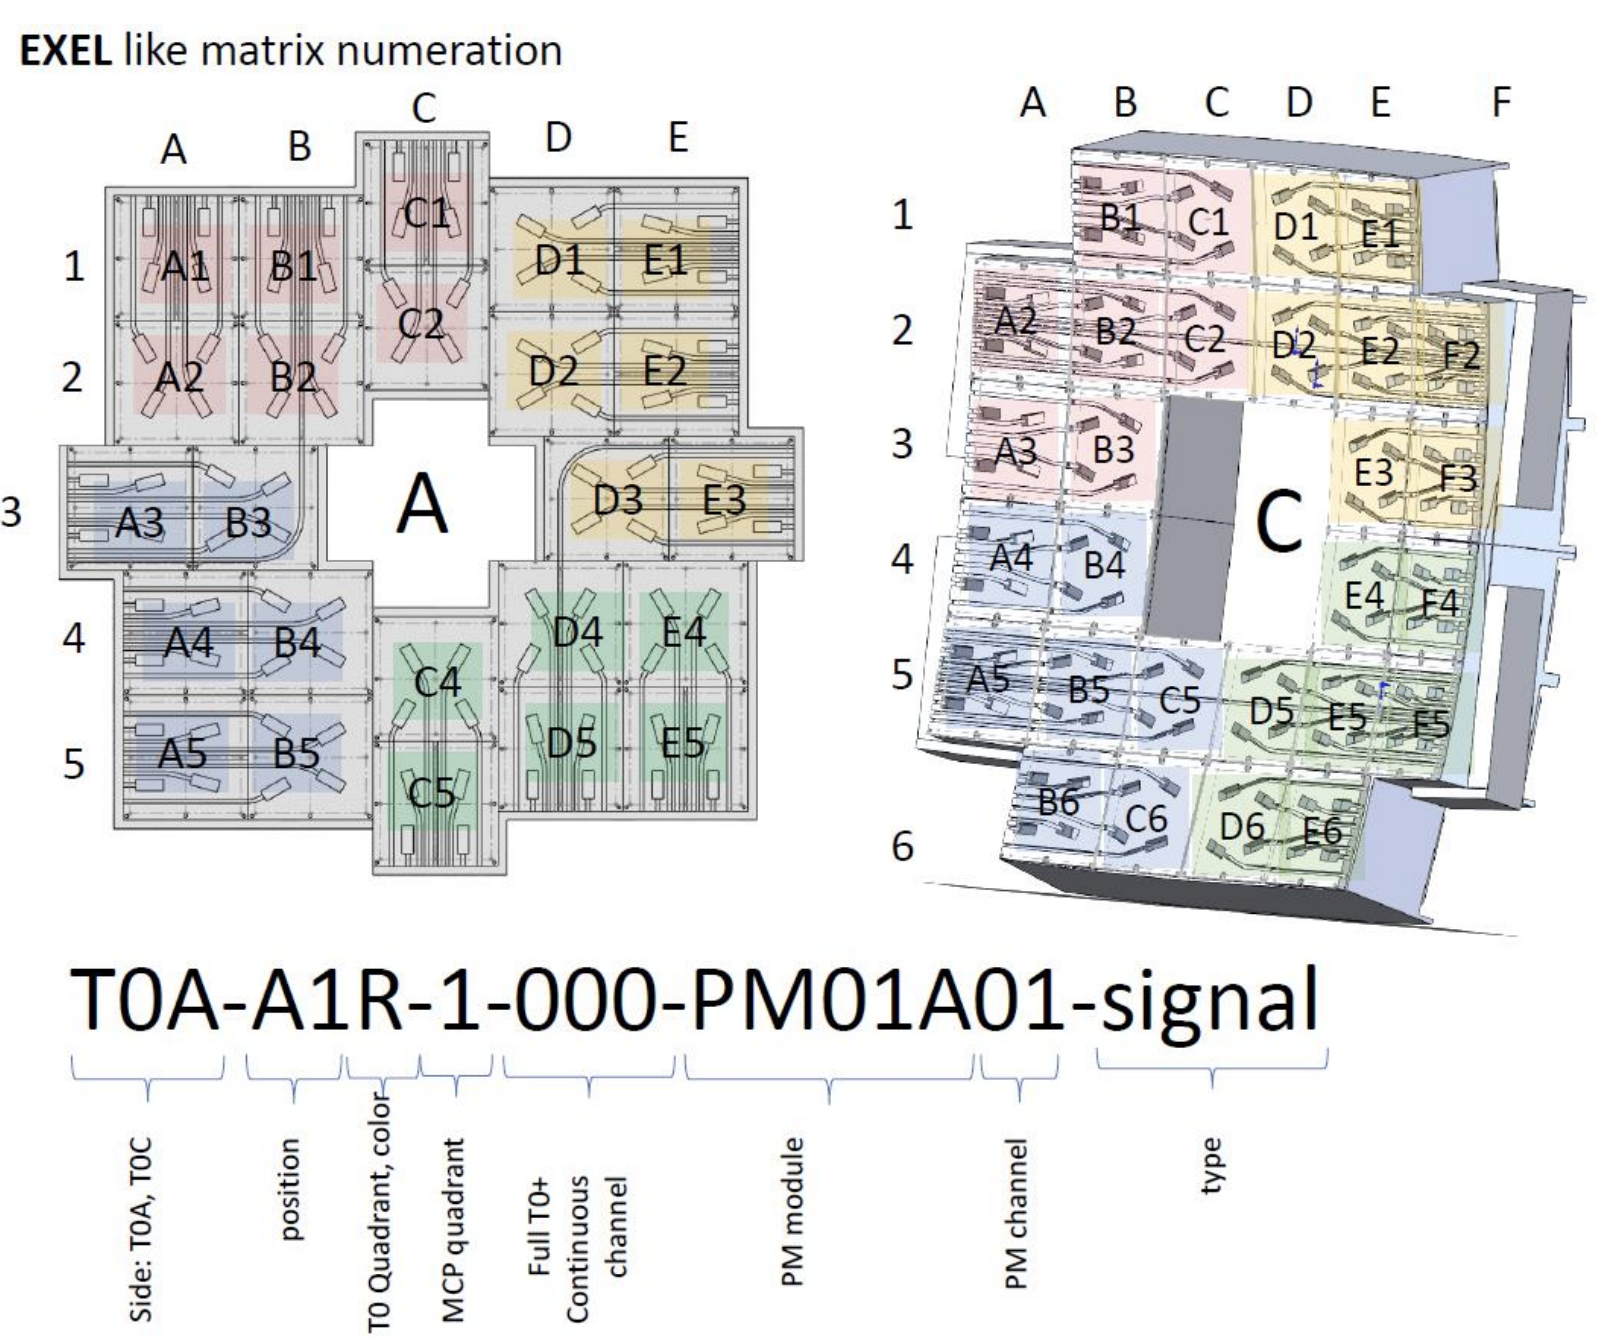
\includegraphics[width=0.6\textwidth]{figures/FIT/T0_Structure_and_Cell_Numbers.png}
    \caption{Aluminum support structure for FT0 A and C sides. Cells are enumerated by row and column.}
    \label{fig:FT0_Labels}
\end{figure}

\section{Results and Discussion}

After the FT0-A detector geometry was completed, a set of simulations of the sensitive components and the support structure for the FT0-A were run, using PYTHIA \cite{PYTHIA} in $O^2$.  Figure \ref{fig:FT0A-SensitiveComponents} shows the geometry of the sensitive components of the A-side detector, including the Cherenkov radiative crystals (Top) and MCP-PMTs (Bottom), coupled with optical grease.  Figure \ref{fig:HitHistogram} shows the location of all simulated hits in those sensitive components, as determined by the particle transport process in GEANT4. The next steps in this analysis include investigating the secondary particles produced in this simulation and evaluating their contribution to the noise in other detectors. This future work is described in Chapter 4.


\begin{figure}[H]
    \centering
    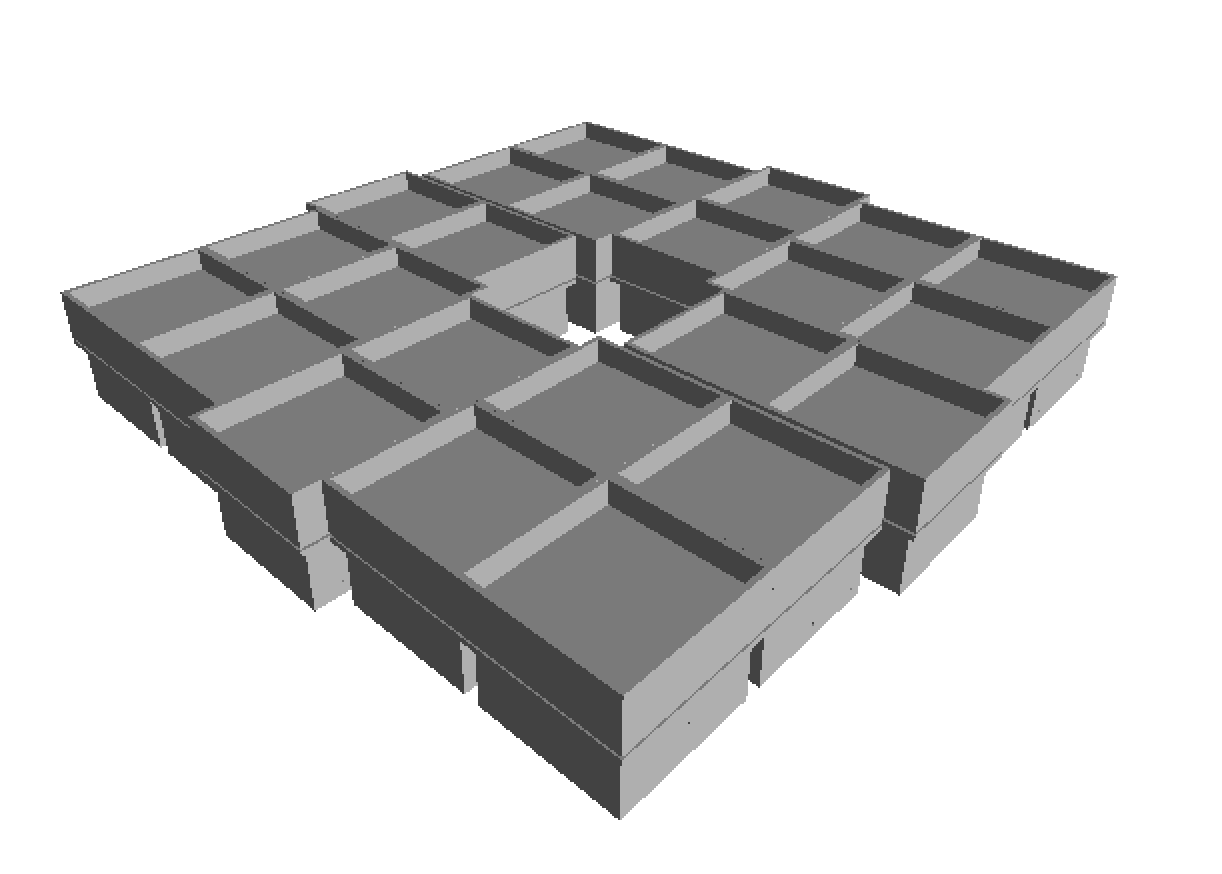
\includegraphics[width=0.8\textwidth]{figures/FIT/T0+_Sensitive_Components.png}
    \caption{Sensitive components for FT0-A. This includes the Cherenkov radiative crystals (Top) and MCP-PMTs (Bottom), coupled with optical grease}
    \label{fig:FT0A-SensitiveComponents}
\end{figure}

\begin{figure}[H]
    \centering
    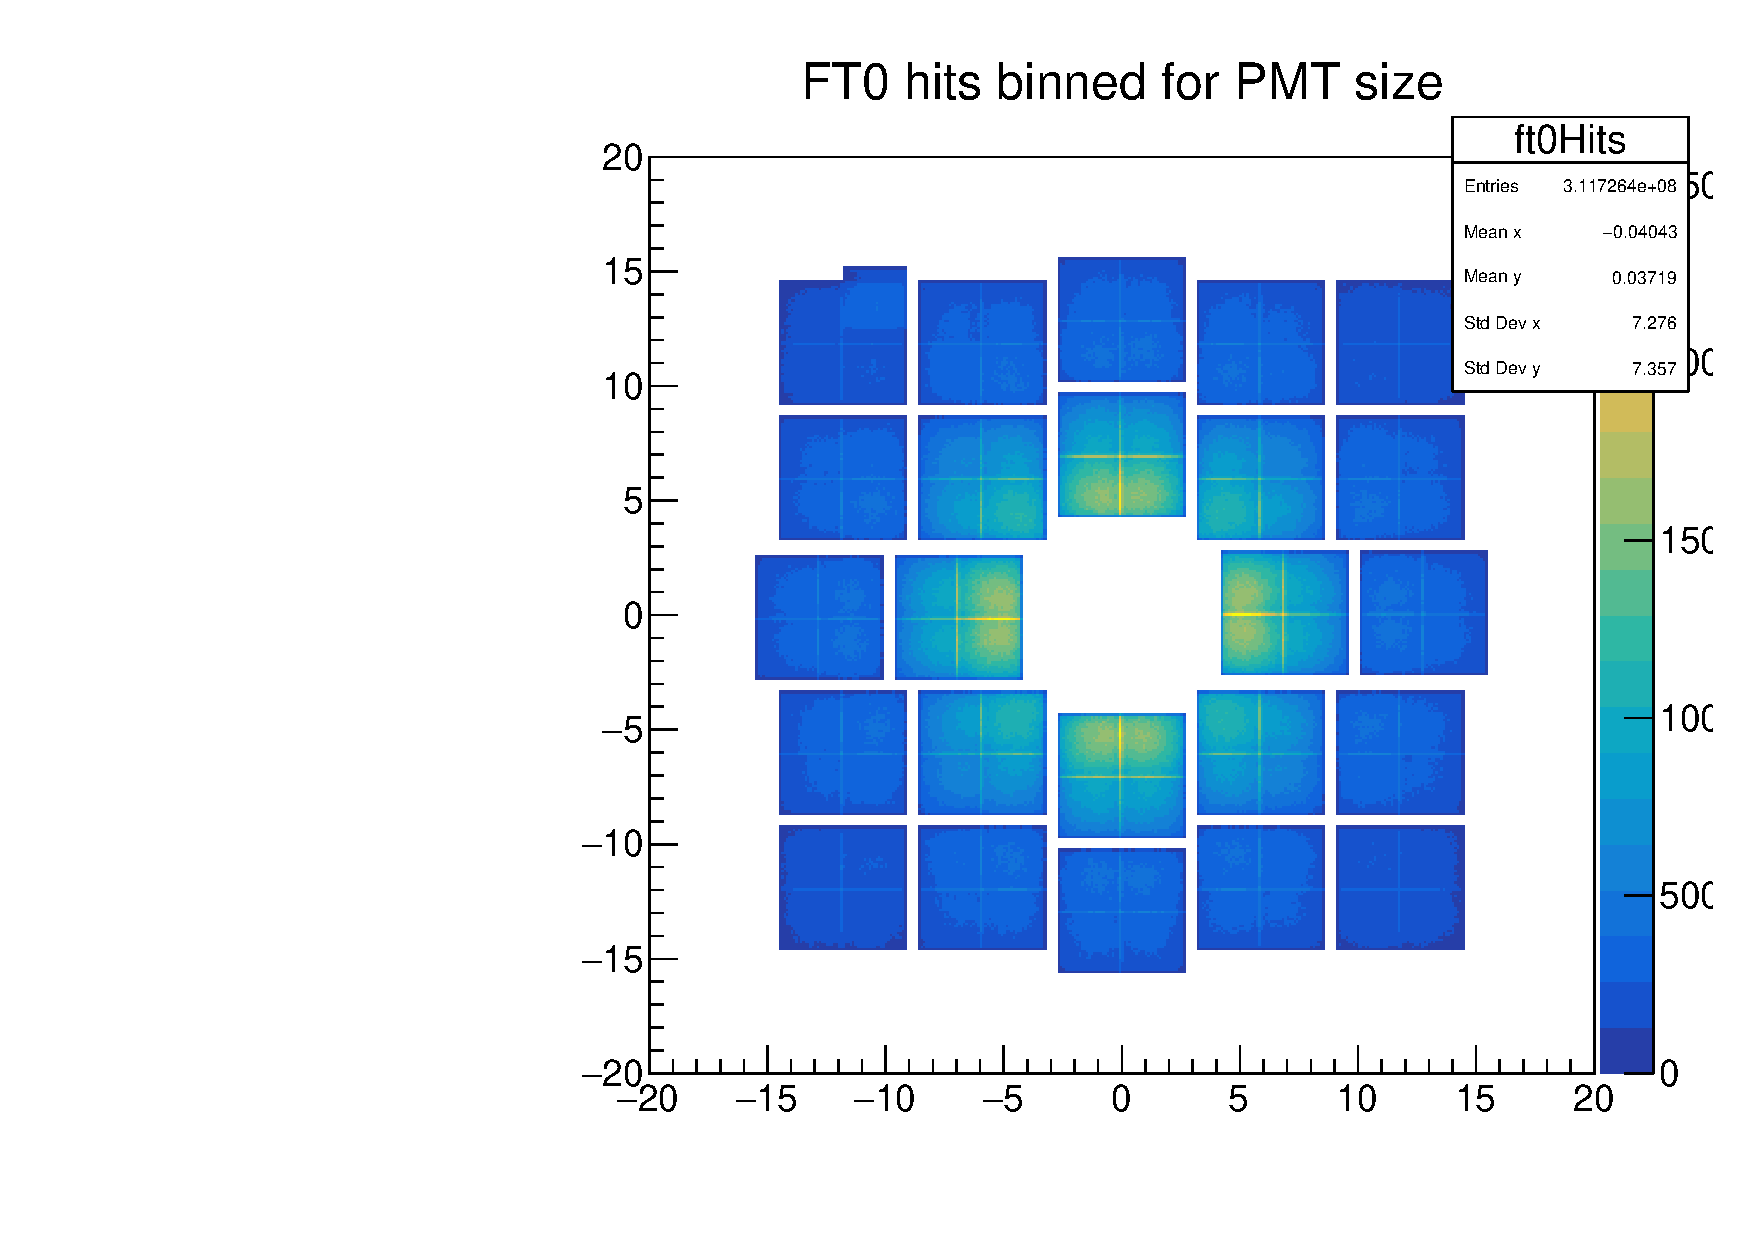
\includegraphics[width= 0.8\textwidth]{figures/analysis/T0+_Sensitive_Components.pdf}
    \caption{Histogram of energy deposited in the FT0-A sensitive components (``hits''), as simulated by GEANT4 particle transport. The MCPs nearest the beamline in p-p collisions end up most exposed due to low transverse momentum interactions.}
    \label{fig:HitHistogram}
\end{figure}
